\documentclass[10pt,journal,compsoc]{IEEEtran}

\usepackage{fontspec}
\usepackage{xeCJK}
\setmainfont{Tinos}
\setsansfont{Arimo}
\setmonofont{Liberation Mono}
\setCJKmainfont[BoldFont=Noto Serif CJK SC Bold]{Noto Serif CJK SC}
\setCJKsansfont[BoldFont=Noto Sans CJK SC Bold]{Noto Sans CJK SC}

\usepackage{amsmath,amssymb}
\usepackage{graphicx}
\graphicspath{{../figures/}}
\usepackage[table]{xcolor}
\usepackage{booktabs,tabularx,array,multirow,makecell}
\usepackage{subcaption}
\usepackage{stfloats}
\usepackage{placeins}
\usepackage{microtype}
\usepackage{enumitem}
\usepackage{url}
\usepackage{cite}
\usepackage{balance}

\definecolor{arrival}{HTML}{4C78A8}
\definecolor{capture}{HTML}{F28E2B}
\definecolor{oneeuro}{HTML}{59A14F}
\definecolor{ours}{HTML}{E15759}
\definecolor{oursbg}{HTML}{FDECEC}
\definecolor{lightgray}{HTML}{F3F4F6}
\definecolor{textgray}{HTML}{5F6670}
\newcommand{\oursname}{\textsc{EgoAnchor}}
\newcommand{\best}[1]{\textbf{\color{ours}#1}}
\newcommand{\notsig}[1]{\color{textgray}#1}
\newcommand{\metric}[2]{\makecell[c]{#1\\[-1pt]{\scriptsize\color{textgray}#2}}}

\setlength{\columnsep}{0.21in}
\setlength{\textfloatsep}{8pt plus 2pt minus 2pt}
\setlength{\floatsep}{7pt plus 2pt minus 2pt}
\setlength{\intextsep}{7pt plus 2pt minus 2pt}
\captionsetup{font=footnotesize,labelfont=bf,skip=3pt}
\captionsetup[sub]{font=scriptsize,labelfont=bf,skip=1pt}
\setlist[itemize]{leftmargin=*,nosep}
\setlist[enumerate]{leftmargin=*,topsep=2pt,itemsep=2pt}

\title{EgoAnchor：面向消费级混合现实的零样本稳定动态物体锚定系统}
\author{匿名作者}

\begin{document}

\IEEEtitleabstractindextext{%
\begin{abstract}
动态真实物体锚定使虚拟内容能够随日常物体的拿取、移动和遮挡持续保持空间附着，是对象中心混合现实应用的基础能力。现有方案通常依赖物理标记、专用追踪设备或受限的平台对象集合。零样本6DoF位姿估计扩大了可被视觉定位的物体范围，但其输出仍是异步、低频且质量波动的相机系位姿观测，无法直接作为混合现实应用的对象锚点。本文提出\oursname，一套面向消费级混合现实的零样本动态物体锚定系统。给定目标物体的三维模型，系统无需物理标记或逐物体训练，通过开放词表初始化、时序分割、双目深度估计和模型驱动的6DoF位姿估计构建对象感知后端；随后以VCD位姿验证和运动状态感知的锚定运行时，将异步观测持续转化为稳定、世界一致且可恢复的对象锚点。我们在Meta Quest 3与外部GPU工作站上实现系统，并通过受控系统基准、组件消融和24人被试内研究进行评价。采集时刻对齐将头动相关误差降低2.69倍，静止锚定将中心化静止误差降低17.06倍；用户研究进一步显示，\oursname 在静止稳定性、位置正确性、恢复一致性、可靠性和依赖意愿方面获得更高评价。
\end{abstract}
\begin{IEEEkeywords}
透视混合现实，动态对象锚定，零样本6DoF位姿估计，运行时系统，用户感知
\end{IEEEkeywords}}

\maketitle

\section{引言}
透视混合现实（Passthrough Mixed Reality, PMR）正在将虚拟内容带到用户身边的真实物体上，用于操作引导、状态可视化、近物交互界面与对象增强。这些应用不仅需要识别物体，还需要一个能够随物体运动持续更新的对象级空间参考：当用户转头、拿起、旋转、放下或短暂遮挡物体时，虚拟内容应保持与物体一致的六自由度（6DoF）关系。传统空间锚点适合静态环境，却不能表达物体自身的运动；动态真实物体锚定因而是对象中心消费级MR的基础系统能力。

现有方案分别覆盖了这一能力的部分环节。物理标记与专用追踪器能够提供稳定位姿，却要求改造目标物体；平台原生对象追踪具有良好系统集成，但其对象范围、模型准备和运行时行为由平台接口限定~\cite{appleObjectAnchor,azureObjectAnchors,vuforiaModelTargets,metaDynamicObjectTracker}。近期的开放词表分割、双目重建和零样本6DoF位姿估计使给定三维模型的更多刚性物体可以被视觉定位~\cite{megapose2022,foundationpose2023}，为无标记对象锚定提供了新的感知基础。

然而，\emph{视觉位姿并不等同于应用可用的MR锚点}。视觉后端输出的是某一历史采集时刻、相机坐标系下的位姿观测；它通常异步到达、更新频率低，并随遮挡、深度噪声和几何错配而波动。若在候选到达时直接与当前头显位姿复合，用户头动会被误写入物体轨迹；若每个候选都直接更新渲染，错误观测会产生跳变，静止噪声会形成持续抖动，而遮挡期间的保持与恢复也缺少明确语义。要将零样本视觉能力用于PMR，需要一个专门的系统层把\emph{位姿观测}转换为\emph{持续锚点}。

本文提出\oursname。系统由零样本对象感知后端和对象锚定运行时组成。感知后端以头显双目图像、目标文本和可用三维模型为输入，组织开放词表初始化、时序分割、米制双目深度与模型驱动6DoF估计，并以VCD（Visibility-gated Color-Depth）评分验证候选。锚定运行时根据图像帧标识恢复采集时刻的相机世界变换，在统一边界接纳可靠观测，并依据物体状态在运动插值、静止锁定与遮挡保持之间切换。由此，系统在不使用物理标签或逐物体训练的前提下，为不受预定义类别集合限制的刚性物体提供世界系、逐渲染帧且带生命周期状态的对象锚点。

\begin{figure*}[t]
  \centering
  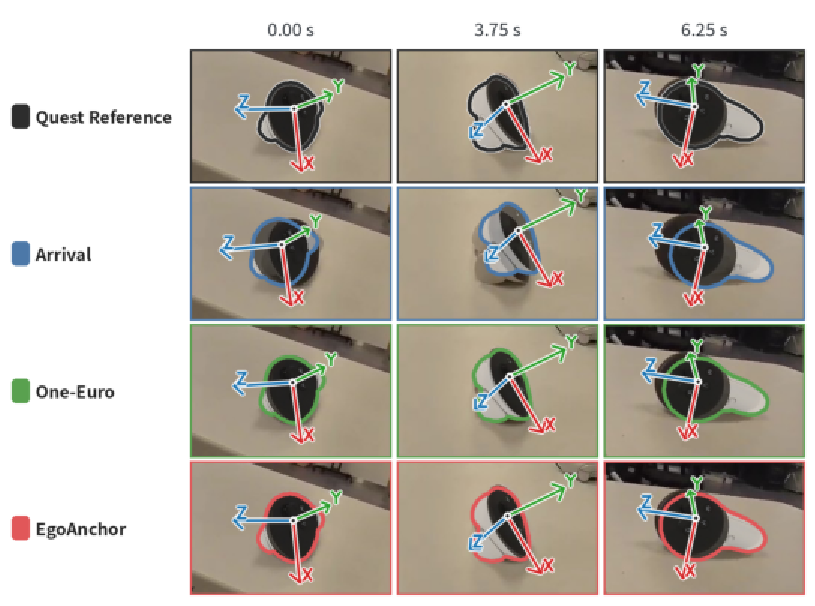
\includegraphics[width=0.94\textwidth]{teaser_sequence.pdf}
  \caption{同一段拿取与旋转序列中的平台参考、朴素到达时刻复合、One-Euro锚点和\oursname。Arrival将头显运动与异步观测混合，One-Euro减弱了波动但仍保留静止漂移；\oursname 在运动后稳定贴合参考。受控评价中，采集时刻对齐将头动相关误差降低2.69倍，StaticLock将中心化静止误差降低17.06倍。}
  \label{fig:teaser}
\end{figure*}

受控评价显示，\oursname 的中心化静止平移泄漏为0.82~mm，平台参考下的绝对注册误差中位数为6.60~mm；相比关闭StaticLock，静止误差降低17.06倍。动态阶段中，系统在360/345~ms的平移/旋转有效时延下获得9.12~mm/4.81$^\circ$的时延对齐残差。24人用户研究进一步表明，参与者对其静止稳定、位置正确、恢复一致和依赖意愿给出更高评分，18/24人更愿意信任\oursname 的锚定结果。

本文的贡献为：
\begin{enumerate}
  \item \textbf{零样本动态物体锚定系统。} 给定目标物体三维模型，\oursname 无需物理标记或逐物体训练，将Quest 3双目图像中的视觉观测转化为应用可持续消费的世界系对象锚点。
  \item \textbf{质量感知的对象锚定方法。} 系统结合VCD位姿验证、采集时刻世界配准和运动状态感知的锚点合成，在静止、运动、短时遮挡与重新获取期间提供明确且可预测的输出行为。
  \item \textbf{分层系统评价。} 我们通过具有平台参考的端到端基准、关键组件消融和24人被试内研究，量化系统性能、解释关键设计的作用，并验证锚点行为差异的感知效用。
\end{enumerate}

\section{相关工作}
\subsection{真实物体追踪与锚定}
基于AprilTag、ArUco等人工标记的方法实现简单且鲁棒~\cite{kato1999artoolkit,olson2011apriltag,garridojurado2014aruco}，但会改变物体外观并约束自然抓握。无标记平台能力逐渐成熟，例如Azure Object Anchors、Vuforia Model Targets以及消费级头显上的对象追踪接口~\cite{azureObjectAnchors,vuforiaModelTargets,appleObjectAnchor,metaDynamicObjectTracker}；这些方案通常依赖平台规定的模型准备流程、支持范围或受控初始化。\oursname 的目标不是替代平台追踪，而是探索一种开放的系统路径：给定可用三维模型，以头显双目视觉和外部通用GPU接入不同类别的日常刚性物体，并向应用暴露锚点位姿与生命周期状态。

\subsection{零样本6DoF位姿估计}
6DoF位姿估计从图像中恢复刚性物体相对于相机的空间位姿。CosyPose、MegaPose等方法通过渲染比较提升未知对象的泛化能力~\cite{cosypose2020,megapose2022}，FoundationPose进一步支持给定三维模型的零样本位姿注册与追踪~\cite{foundationpose2023}。开放词表目标检测、视频对象分割和立体匹配则分别提供语义初始化、稳定掩膜和米制几何。上述研究主要优化相机系位姿本身；\oursname 关注如何组织这些模块，并把异步候选转换为应用侧动态锚点。

\subsection{XR时延与含噪输入处理}
配准误差和端到端时延长期影响AR/VR体验~\cite{azuma1994improving,diluca2010latency}。头部位姿预测和异步时间扭曲主要处理设备与显示链路~\cite{vanwaveren2016atw}，One-Euro等滤波器则在交互输入中权衡抖动与延迟。异步视觉对象位姿具有不同的时间语义：候选属于历史图像时刻，其世界关系必须结合设备历史位姿恢复；同时，应用还需要定义观测之间、遮挡期间以及重新获取时的锚点行为。\oursname 将这些职责统一到对象锚定运行时中。

\section{EgoAnchor系统}
\subsection{系统概览与数据契约}
\oursname 将系统分为对象感知后端和对象锚定运行时（图~\ref{fig:overview}）。感知后端生成观测
\begin{equation}
 o_f=\left(f,t_f,T_o^{c_f},R_f\right),
\end{equation}
其中$f$和$t_f$分别为图像帧标识与采集时间，$T_o^{c_f}\in\mathrm{SE}(3)$为物体相对于采集相机的位姿，$R_f\in[0,1]$为即时可靠性评分。运行时输出
\begin{equation}
 a(t)=\left(T_o^w(t),s(t),u(t)\right),
\end{equation}
即渲染时刻的世界系锚点、生命周期状态和可用性状态。该契约将低频异步的视觉观测与逐帧MR应用解耦，也使应用可以根据Tracked、Stationary、Frozen或Lost状态决定显示、冻结或重新注册策略。

\begin{figure*}[t]
  \centering
  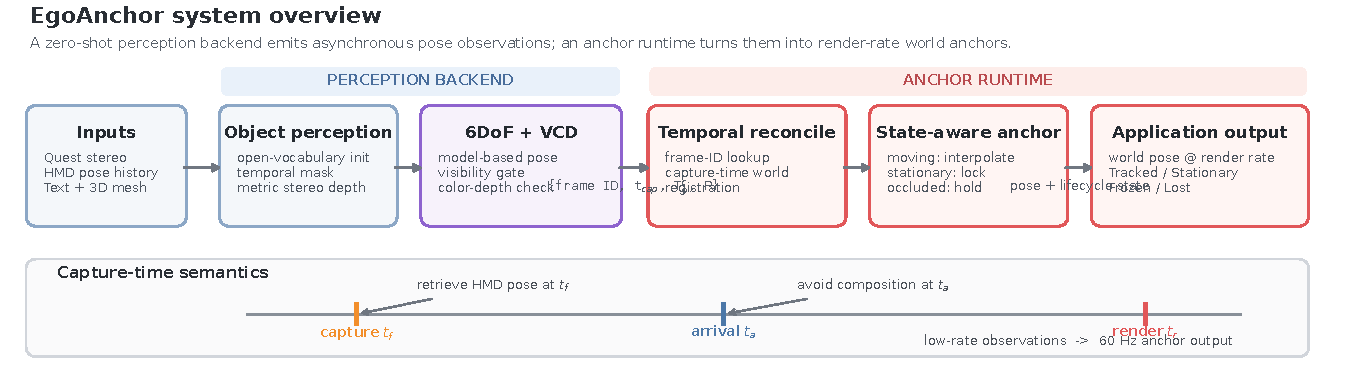
\includegraphics[width=0.97\textwidth]{system_overview.pdf}
  \caption{\oursname 的分层架构。感知后端输出带帧标识、采集时间和可靠性证据的相机系6DoF观测；锚定运行时恢复采集时刻世界关系，并根据观测质量与物体状态持续合成世界系锚点。底部时间线强调：历史视觉观测应与采集时刻$t_f$的相机位姿复合，而不是与候选到达时刻$t_a$复合。}
  \label{fig:overview}
\end{figure*}

\subsection{零样本对象感知}
为在无需逐物体训练的条件下接入新目标，感知后端采用四阶段流水线。开放词表检测以目标文本建立初始掩膜；视频对象分割在后续帧中传播目标区域；双目立体匹配恢复米制深度；FoundationPose接收目标三维模型、掩膜和深度，在初始化阶段执行全局注册，在追踪阶段以历史位姿为先验迭代优化。四个模块分别提供语义、时间连续性、尺度和三维对齐，共同输出相机系6DoF候选。

\subsection{VCD位姿验证}
弱纹理、遮挡和深度噪声可能使位姿估计器输出形式合法但物理错误的候选。VCD将目标模型按候选位姿渲染回图像空间，并从可视度、颜色投影和深度几何三类证据验证候选：
\begin{equation}
R=V\cdot G_{\mathrm{CD}},\qquad
G_{\mathrm{CD}}=\exp\!\left(\frac{w_C\ln\max(C,\epsilon)+w_D\ln\max(D,\epsilon)}{w_C+w_D}\right).
\end{equation}
$V$为渲染投影被观测掩膜支持的比例，$C$和$D$分别衡量颜色投影与深度结构一致性。几何均值使任一模态明显不一致时评分迅速下降；运行时只接纳评分超过相应状态阈值的观测。具体通道实现和参数列于补充材料。

\subsection{运动状态感知的锚定运行时}
\subsubsection{采集时刻世界配准}
候选到达时已经滞后于其图像采集时刻。运行时在采集阶段缓存帧标识$f$及相机世界变换$T_c^w(f)$；观测到达后以
\begin{equation}
T_o^w(f)=T_c^w(f)\,T_o^{c_f}
\label{eq:world}
\end{equation}
恢复观测在原始采集时刻的世界关系。该步骤消除由采集到到达之间的头显运动造成的坐标错配。随后，VCD接纳的世界系观测进入状态估计。

\subsubsection{连续运动与静止锁定}
低频且不规则的观测不能直接驱动逐帧渲染。系统以常速度卡尔曼模型估计平移、旋转及其速度，并在略滞后的目标时间上，仅在已到达控制点之间对位置进行线性插值、对旋转执行SLERP。与直接外推相比，这一策略优先避免噪声放大和错误预测。

固定参数平滑无法同时满足静止稳定和运动响应。\oursname 因此根据物体状态改变锚点生成策略：当线速度、角速度和可靠性在驻留窗口内持续满足静止条件时，运行时将输出锁定到稳定参考；持续运动、累积位移或可靠性变化触发解锁，控制权返回连续轨迹。该策略并非消除稳定性--响应性权衡，而是将其显式分配到不同运动状态。

\subsubsection{遮挡与生命周期}
运行时根据距离最近可靠观测的时间维护Tracked、Stationary、FrozenUncertain和Lost状态。短时失去观测时，系统停止吸收低分候选并保持最后可靠锚点；观测恢复后，只有连续可靠的候选才能重新进入状态估计。本实验的统一遮挡阶段均进入FrozenUncertain并在遮挡解除后自动恢复，从而避免低质量重检测直接产生可见跳变。

\section{系统实现}
Quest 3端以Unity和Meta XR接口采集双目透视图像、相机标定和设备位姿历史，并以约60~Hz更新对象锚点；外部RTX~3090工作站运行开放词表检测、Cutie时序分割、Fast-FoundationStereo、FoundationPose和VCD渲染验证。头显与工作站通过Wi-Fi~6局域网异步通信，高带宽图像流采用最新帧优先，低带宽位姿与状态消息独立传输。受控批次中，服务器追踪处理时间中位数为77.36~ms，候选发布间隔中位数为106.74~ms（约9.37~Hz）。实现参数、软件版本和完整状态阈值移至补充材料，以便正文聚焦影响锚点行为的系统设计。

\section{系统评估}
评价遵循“完整系统行为--组件归因--感知效用”的证据链。实验一在平台参考下比较四种锚定配置，刻画头动、静止、持续运动、起停转换与遮挡期间的端到端行为；实验二在同一候选流上切换单一设计，解释性能来源；实验三以三种日常刚性物体开展被试内研究，检验锚点行为差异是否被用户感知并影响信任。

\subsection{受控设置与比较方法}
受控评价以Quest Touch Plus控制器为视觉目标，并以平台SDK的控制器6DoF位姿作为同步参考。该参考与头显共享平台世界坐标系，适合比较同一时间线上的不同运行时，但不等同于外部光学真值。所有配置消费相同的相机系候选、采集和到达时间、渲染时间线及参考轨迹。

\textbf{Arrival}在候选到达时使用当前头显位姿完成世界复合并保持；\textbf{Capture}改用采集时刻复合；\textbf{One-Euro}在采集时刻对齐和VCD接纳后采用One-Euro平滑及同一历史插值；\textbf{EgoAnchor}采用卡尔曼状态估计、历史Linear/SLERP合成、StaticLock和生命周期管理。

\clearpage
\subsection{实验一：应用侧锚点行为}
图~\ref{fig:exp1}以统一视觉语法展示四种配置的误差与残余抖动。静止阶段，\oursname 的中心化平移泄漏和帧间增量分别为0.82~mm与0.06~mm，明显低于One-Euro的10.65~mm与0.85~mm；平台参考下绝对注册误差中位数为6.60~mm。遮挡期间的平移P95为4.85~mm。代价是从静止锁定转入运动输出的中位转换时间增加至510~ms，表明系统采用稳定优先的起停策略。

持续运动中，\oursname 的平移/旋转有效时延为360/345~ms，时延对齐RMSE为9.12~mm/4.81$^\circ$，优于One-Euro的15.69~mm/5.55$^\circ$。这些量必须联合解释：对齐RMSE描述移除相位差后的轨迹保真度，而同一渲染时刻的误差仍包含系统延迟。表~\ref{tab:summary}集中给出主结果，完整IQR和current-time RMSE列于补充材料。

\begin{figure*}[t]
  \centering
  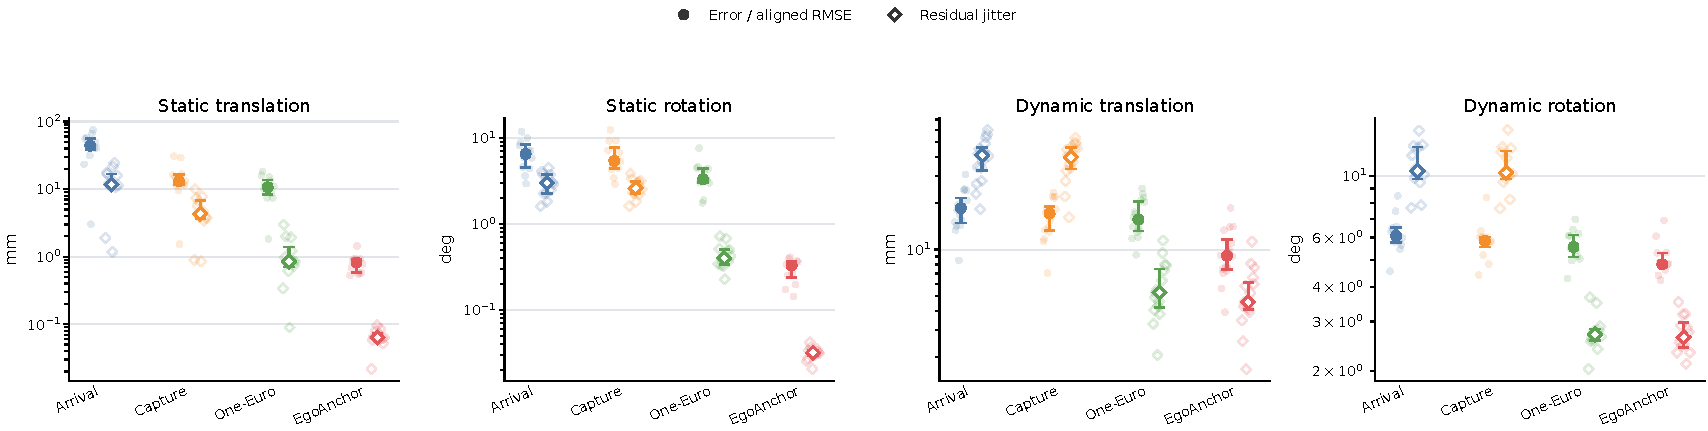
\includegraphics[width=0.98\textwidth]{exp1_behavior.pdf}
  \caption{实验一的静止与动态锚点行为。颜色在全文中固定表示四种方法；实心圆表示静止误差或时延对齐RMSE，空心菱形表示对应残余抖动。淡色点为片段，粗标记为中位数与IQR。纵轴采用对数刻度以同时呈现亚毫米静止波动和厘米级基线误差。}
  \label{fig:exp1}
\end{figure*}

\begin{table*}[t]
\centering
\caption{实验一的关键系统行为（片段间中位数，越低越好）。动态时延与时延对齐RMSE应联合解释；完整IQR见补充材料。浅红底标记完整系统。}
\label{tab:summary}
\small
\setlength{\tabcolsep}{5.0pt}
\renewcommand{\arraystretch}{1.12}
\begin{tabular}{lcccccc}
\toprule
方法 & \makecell{头动泄漏\\P95 (mm)} & \makecell{静止增量\\P95 (mm)} & \makecell{遮挡误差\\P95 (mm)} & \makecell{起动转换\\(ms)} & \makecell{动态对齐RMSE\\平移/旋转} & \makecell{有效时延\\平移/旋转 (ms)} \\
\midrule
Arrival & 43.67 & 11.70 & 18.23 & \textbf{157} & 18.57~mm / 6.09$^\circ$ & \textbf{203 / 255} \\
Capture & 13.03 & 4.30 & 16.93 & 264 & 17.14~mm / 5.84$^\circ$ & 255 / 258 \\
One-Euro & 10.65 & 0.85 & 10.41 & 334 & 15.69~mm / 5.55$^\circ$ & 380 / 385 \\
\rowcolor{oursbg}\textbf{EgoAnchor} & \best{0.82} & \best{0.06} & \best{4.85} & 510 & \best{9.12~mm / 4.81$^\circ$} & 360 / 345 \\
\bottomrule
\end{tabular}
\end{table*}

\clearpage

\subsection{实验二：关键设计归因}
图~\ref{fig:exp2}表明，系统性能并非来自单一滤波器。首先，同一视觉候选按到达时刻而非采集时刻复合时，头动相关误差增加2.69倍，说明历史时间语义是世界一致性的前提。其次，关闭StaticLock使静止误差增加17.06倍，且12/12片段均变差。第三，VCD的风险排序将event级选择风险从7.25~mm降至4.79~mm，12/12个event均获得正收益。最后，在关闭StaticLock的公平条件下，向当前时刻外推的Smoothed KF相较历史Linear/SLERP插值产生5.46倍平移残差和2.63倍旋转残差；在当前候选频率和噪声水平下，保守的历史合成更可靠。

\begin{figure*}[t]
  \centering
  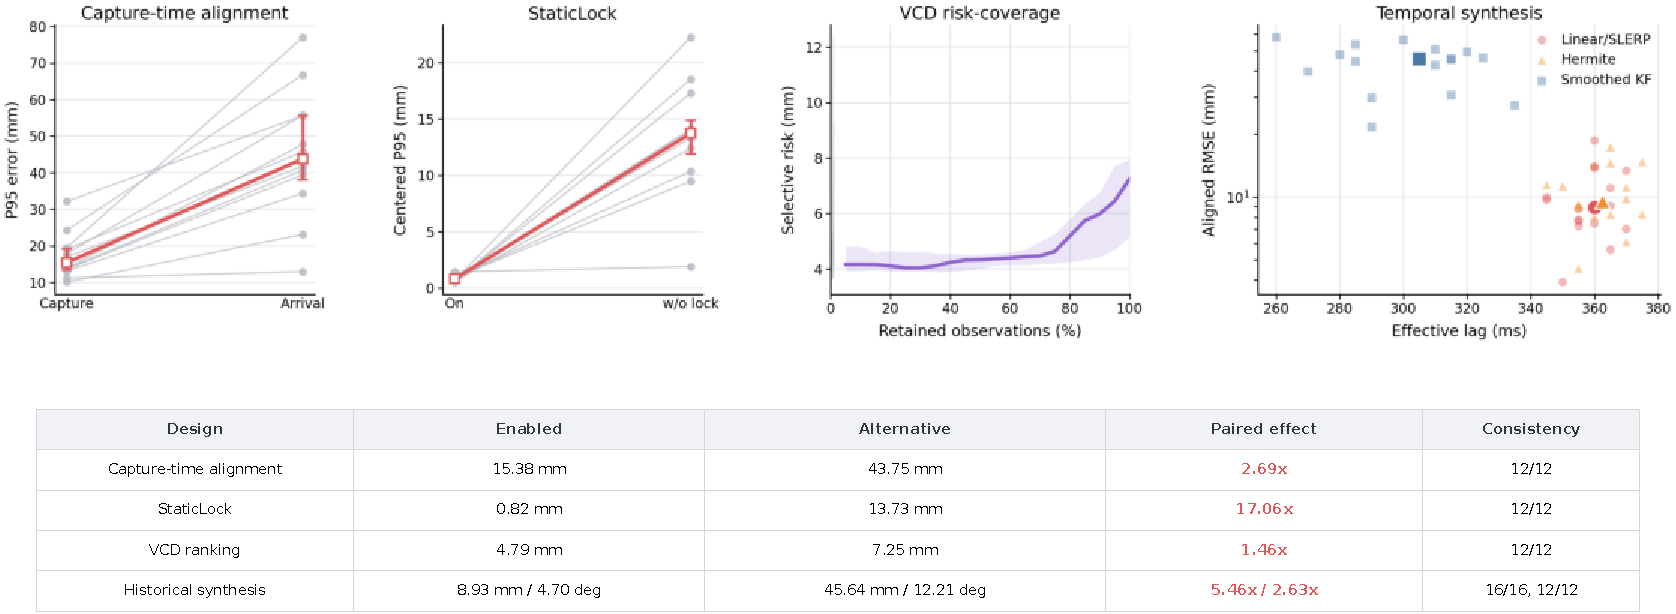
\includegraphics[width=0.98\textwidth]{exp2_combined.pdf}
  \caption{实验二的组件归因与紧凑结果汇总。前两幅图以配对斜率显示每个片段，红色粗线为中位数与IQR；VCD图展示保留率--风险关系；时序策略图联合显示有效时延和时延对齐平移RMSE。底部表格给出启用设计、关闭或替代方案、配对效应倍率及一致性。}
  \label{fig:exp2}
\end{figure*}

\subsection{实验三：日常物体上的感知效用}
\subsubsection{设计与测量}
研究采用$2\times3$完全被试内设计，比较One-Euro与\oursname 在无线鼠标、闭合订书机和游戏手柄上的表现。每个方法--物体条件依次包含静止观察、拿起--移动--放置以及完全遮挡--恢复三个阶段，分别暴露世界一致性与抖动、运动附着与起停转换、遮挡保持与重新获取。完成每个条件后，参与者评价静止稳定、运动附着、姿态一致、恢复一致、位置正确、依赖意愿及稳定--响应平衡，并填写AQ子量表；全部条件结束后，对两种方法填写adapted TiA与S-TIAS。配对比较采用双侧Wilcoxon符号秩检验，并在预先冻结的两个家族内作Holm校正。

24名参与者完成全部144个方法--物体区块，其中女性12名、男性12名，年龄$27.08\pm4.45$岁；22名为右利手、2名为左利手，无技术故障导致的区块排除。

\subsubsection{结果}
图~\ref{fig:exp3}和表~\ref{tab:user}显示，\oursname 在静止稳定（$\Delta\mathrm{Mdn}=1.00$）、位置正确（0.67）、恢复一致（0.67）、依赖意愿（1.00）和稳定--响应平衡（0.33）上显著优于One-Euro；运动附着与姿态一致未检出校正后差异。已发表量表中，AQ嵌入质量、TiA可靠性/能力、TiA理解/可预测性和S-TIAS信任均更高，AQ交互质量无显著差异。

最终选择中，15/24人总体偏好\oursname，18/24人更愿意信任其锚定结果；区分信心中位数为6.00 [5.00, 7.00]。开放题中，静止稳定（17/24）和遮挡恢复（11/24）是最常被识别的差异；抖动与漂移（19/24）以及恢复后错位（13/24）是最常导致信任下降的现象。这些结果说明，运行时带来的稳定性和恢复行为不仅反映在系统指标中，也直接影响用户是否愿意依赖对象锚点。

\begin{figure*}[t]
  \centering
  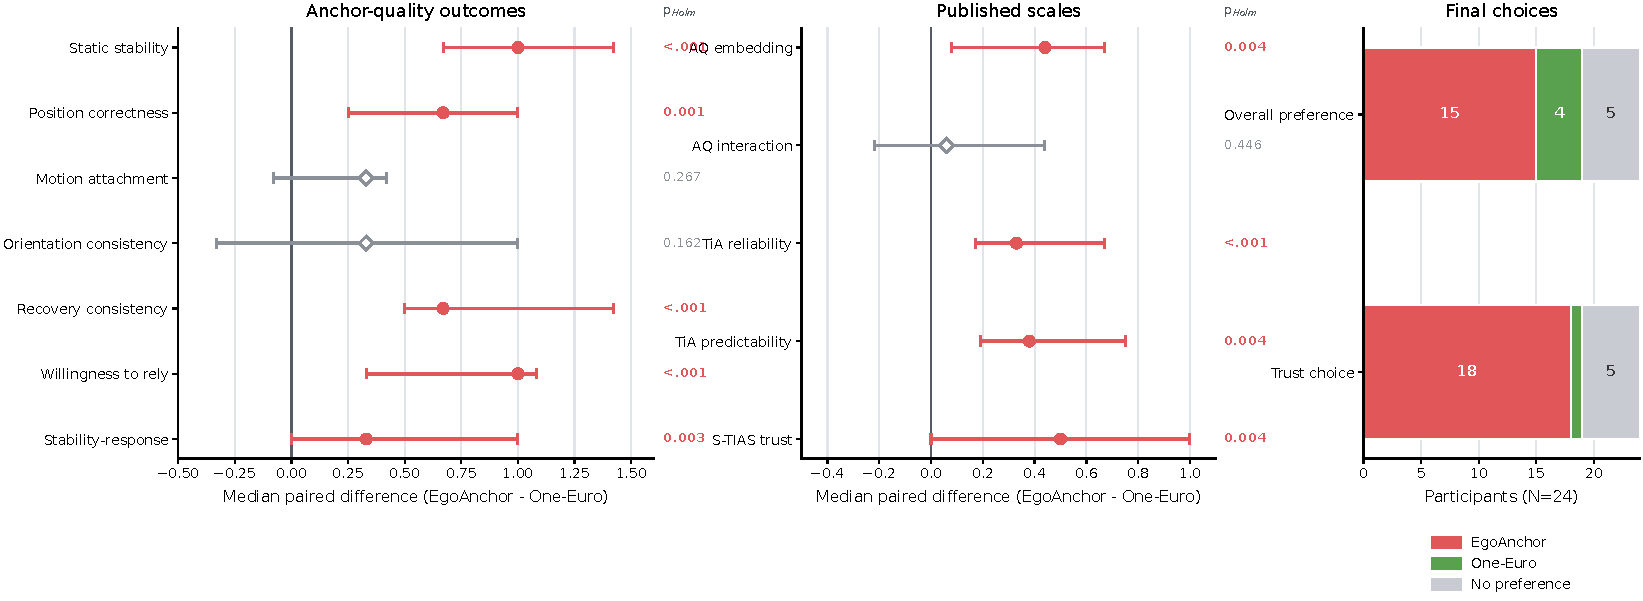
\includegraphics[width=0.98\textwidth]{exp3_perception.pdf}
  \caption{实验三的感知结果。左、中：EgoAnchor减One-Euro的配对差中位数与IQR；红色表示Holm校正后显著，灰色空心标记表示未检出差异。右：总体偏好和信任选择的人数分布。}
  \label{fig:exp3}
\end{figure*}

\begin{table}[t]
\centering
\caption{主证实结局的参与者内比较。}
\label{tab:user}
\footnotesize
\setlength{\tabcolsep}{3.4pt}
\begin{tabular}{lccc}
\toprule
结局 & $\Delta$Mdn & $p_{\mathrm{Holm}}$ & $r_{rb}$ \\
\midrule
静止稳定 & \best{1.00} & \best{$<.001$} & 0.90 \\
位置正确 & \best{0.67} & \best{.001} & 0.85 \\
运动附着 & \notsig{0.33} & \notsig{.267} & 0.29 \\
姿态一致 & \notsig{0.33} & \notsig{.162} & 0.41 \\
恢复一致 & \best{0.67} & \best{$<.001$} & 0.95 \\
依赖意愿 & \best{1.00} & \best{$<.001$} & 0.87 \\
稳定--响应平衡 & \best{0.33} & \best{.003} & 0.90 \\
\bottomrule
\end{tabular}
\end{table}


\section{讨论}
\subsection{系统层贡献：从视觉候选到对象锚点}
\oursname 的主要价值并非单独提出一种位姿估计器或滤波器，而是把零样本对象感知、质量验证和应用侧锚定组织为一套完整系统。输入端允许给定三维模型的新刚性物体在不训练专用网络的情况下接入；输出端不只提供位姿，还提供逐渲染帧更新与生命周期状态。该分层使感知模型可以独立替换，同时保持应用对锚点语义的稳定预期。

\subsection{稳定性、响应性与信任}
StaticLock以更长的起动转换换取放置后的稳定保持，因此适合拿取--放置--读取、对象标注和状态可视化等“运动后消费”任务；对持续快速运动的对象，当前时刻相位误差仍是主要限制。用户研究中的运动附着和AQ交互质量未显著改善，与这一系统边界一致。另一方面，静止稳定和恢复一致显著提高，并成为参与者最常提及的差异，说明对象锚点的可信度取决于完整生命周期，而不只是运动阶段的单一RMSE。

\subsection{适用范围与局限}
系统要求目标具有可用三维模型，并依赖物体在RGB与双目深度中的可观测性；透明、镜面、极弱纹理、严重遮挡和超出有效深度量程仍会削弱分割、几何重建和位姿验证。三种用户研究物体证明了跨类别可用性，但不足以支持“任意日常物体”的泛化结论；更系统的对象覆盖、初始化成功率和接入时间评价仍需补充。受控实验使用平台控制器位姿作为参考，无法观测平台共同漂移，故本文报告的是平台参考下的相对系统行为，而非外部光学真值。系统目前依赖外部GPU工作站和局域网；端侧推理与更低时延的当前时刻预测是后续工作。量表方面，One-Euro条件下AQ交互质量与TiA理解/可预测性的内部一致性偏低，因此相关非显著结果应谨慎解释。

\section{结论}
本文提出\oursname，一套面向消费级混合现实的零样本稳定动态物体锚定系统。系统组织开放词表与模型驱动视觉模块生成6DoF候选，以VCD验证观测质量，并通过采集时刻世界配准、运动状态感知的时序合成和生命周期管理，持续输出世界系对象锚点。受控基准和消融表明，时间语义、观测接纳与状态相关输出共同决定锚点行为；用户研究进一步显示，静止稳定和恢复一致直接影响用户信任。\oursname 因而展示了一条从通用视觉感知到应用可用对象锚点的完整系统路径。

\begin{thebibliography}{14}
\bibitem{appleObjectAnchor} Apple Developer Documentation. ObjectAnchor, 2024.
\bibitem{azuma1994improving} R. Azuma and G. Bishop. Improving static and dynamic registration in an optical see-through HMD. \emph{SIGGRAPH}, 1994.
\bibitem{diluca2010latency} M. Di Luca. New method to measure end-to-end delay of virtual reality. \emph{Presence}, 19(6):569--584, 2010.
\bibitem{garridojurado2014aruco} S. Garrido-Jurado et al. Automatic generation and detection of highly reliable fiducial markers under occlusion. \emph{Pattern Recognition}, 47(6):2280--2292, 2014.
\bibitem{kalman1960new} R. E. Kalman. A new approach to linear filtering and prediction problems. \emph{Journal of Basic Engineering}, 82(1):35--45, 1960.
\bibitem{kato1999artoolkit} H. Kato and M. Billinghurst. Marker tracking and HMD calibration for a video-based augmented reality conferencing system. \emph{IWAR}, 1999.
\bibitem{cosypose2020} Y. Labb\'e et al. CosyPose: Consistent multi-view multi-object 6D pose estimation. 2020.
\bibitem{megapose2022} Y. Labb\'e et al. MegaPose: 6D pose estimation of novel objects via render and compare. 2022.
\bibitem{metaDynamicObjectTracker} Meta. Dynamic Object Tracker documentation, 2025.
\bibitem{azureObjectAnchors} Microsoft Learn. Azure Object Anchors overview, 2026.
\bibitem{olson2011apriltag} E. Olson. AprilTag: A robust and flexible visual fiducial system. \emph{ICRA}, 2011.
\bibitem{vuforiaModelTargets} PTC Vuforia. Model Targets documentation, 2026.
\bibitem{vanwaveren2016atw} J. M. P. van Waveren. The asynchronous time warp for virtual reality on consumer hardware. \emph{VRST}, 2016.
\bibitem{foundationpose2023} B. Wen et al. FoundationPose: Unified 6D pose estimation and tracking of novel objects. 2023.
\end{thebibliography}

\end{document}
